\documentclass[10pt,twocolumn,twoside,slovak,a4paper]{article}

\usepackage[slovak]{babel}
\usepackage[IL2]{fontenc} 
\usepackage[utf8]{inputenc}
\usepackage{graphicx}
\usepackage{url}
\usepackage{hyperref}
\usepackage{cite}

\pagestyle{headings}

\title{Algoritmy odporúčania filmov v Netflix\thanks{Semestrálny projekt v predmete Metódy inžinierskej práce, ak. rok 2024/25, vedenie: Ing. Richard Marko, PhD}}

\author{Yehor Bohuslavskyi\\[2pt]
	{\small Slovenská technická univerzita v Bratislave}\\
	{\small Fakulta informatiky a informačných technológií}\\
	{\small \texttt{xbohuslavkyi@stuba.sk}}
	}

\date{\small 3. oktober 2024}

\begin{document}

\maketitle

\begin{abstract}
Túto tému som si vybral, pretože je veľmi zaujímavé, ako technológie a umelá inteligencia(ktorá je v súčasnosti jednou z najrozvíjajúcejších sa tém) ovplyvňujú naše každodenné rozhodovanie o tom, čo sledujeme. Ja som zvedavý, že ako po zhliadnutí jedného tureckého filmu, ktorý som ani neohodnotil, sa mi v odporúčaniach začali objavovať podobné filmy. 

V systéme sa nachádza viac, ako 15 000 filmov a zobrazuje vám len tie, ktoré sa vám budú páčiť (neskôr dozvieme sa, ako to funguje). Fakt: ani jeden používateľ Netflix nebol by schopný si samostatne nájsť film alebo seriál, ktorý by sa mu páčil bez požívania algoritmu odporúčania filmov \cite{netflixRecAlgorithm}.
 
V tomto článku sa podrobne pozrieme na algoritmy spoločnosti Netflix. V súčasnosti je systém Netflix postavený na algoritme, ktorý využíva umelú inteligenciu a strojové učenie. Pozrieme sa aj na umiestnenie odporúčaní na obrazovke, kde je niekoľko typov návrhov. Prvým je „Odporúčané pre vás“, po ňom idú „Trendy“, na stránke sa nachádza aj záložka „New Releases“.

Podrobne sa pozrieme aj na filtračné algoritmy, ktoré sa delia na dva hlavné typy. Akú rolu odohrávajú hodnotenia a správania používateľov v rámci algoritmu collaborative filtering a „filtrovanie na základe obsahu“.

Zaujímavým aspektom sú aj systémy hodnotenia. Patrí medzi ne „Personalizované hodnotenie videa (PVR)“, „Top-N Ranking“, „Rebríček obľúbených filmov“ a „Zoznam zaujímavého obsahu na neskoršie sledovanie“. Každé z týchto hodnotení je personalizované pre jednotlivých používateľov, čo je veľmi zaujímavé.

V rámci článku sa budeme venovať aj typom údajov, ktoré Netflix používa. Tie sa zhruba delia na dva typy: základné typy zhromažďovaných údajov a dodatočné informácie. Medzi základné patria „interakcie používateľa so stránkou“, ktoré pozostávajú z histórie sledovania a hodnotení. Druhým typom sú „korelačné údaje“, „informácie o obsahu knižnice Netflix“, ako napríklad žánre. Ďalšie uvidíme ako ovplyvňujú  špecifickejšie typy informácií, ako sú napríklad denný čas, používané zariadenie alebo priemerná dĺžka sledovania.

\end{abstract}

\begin{figure}[h!]
  \centering
  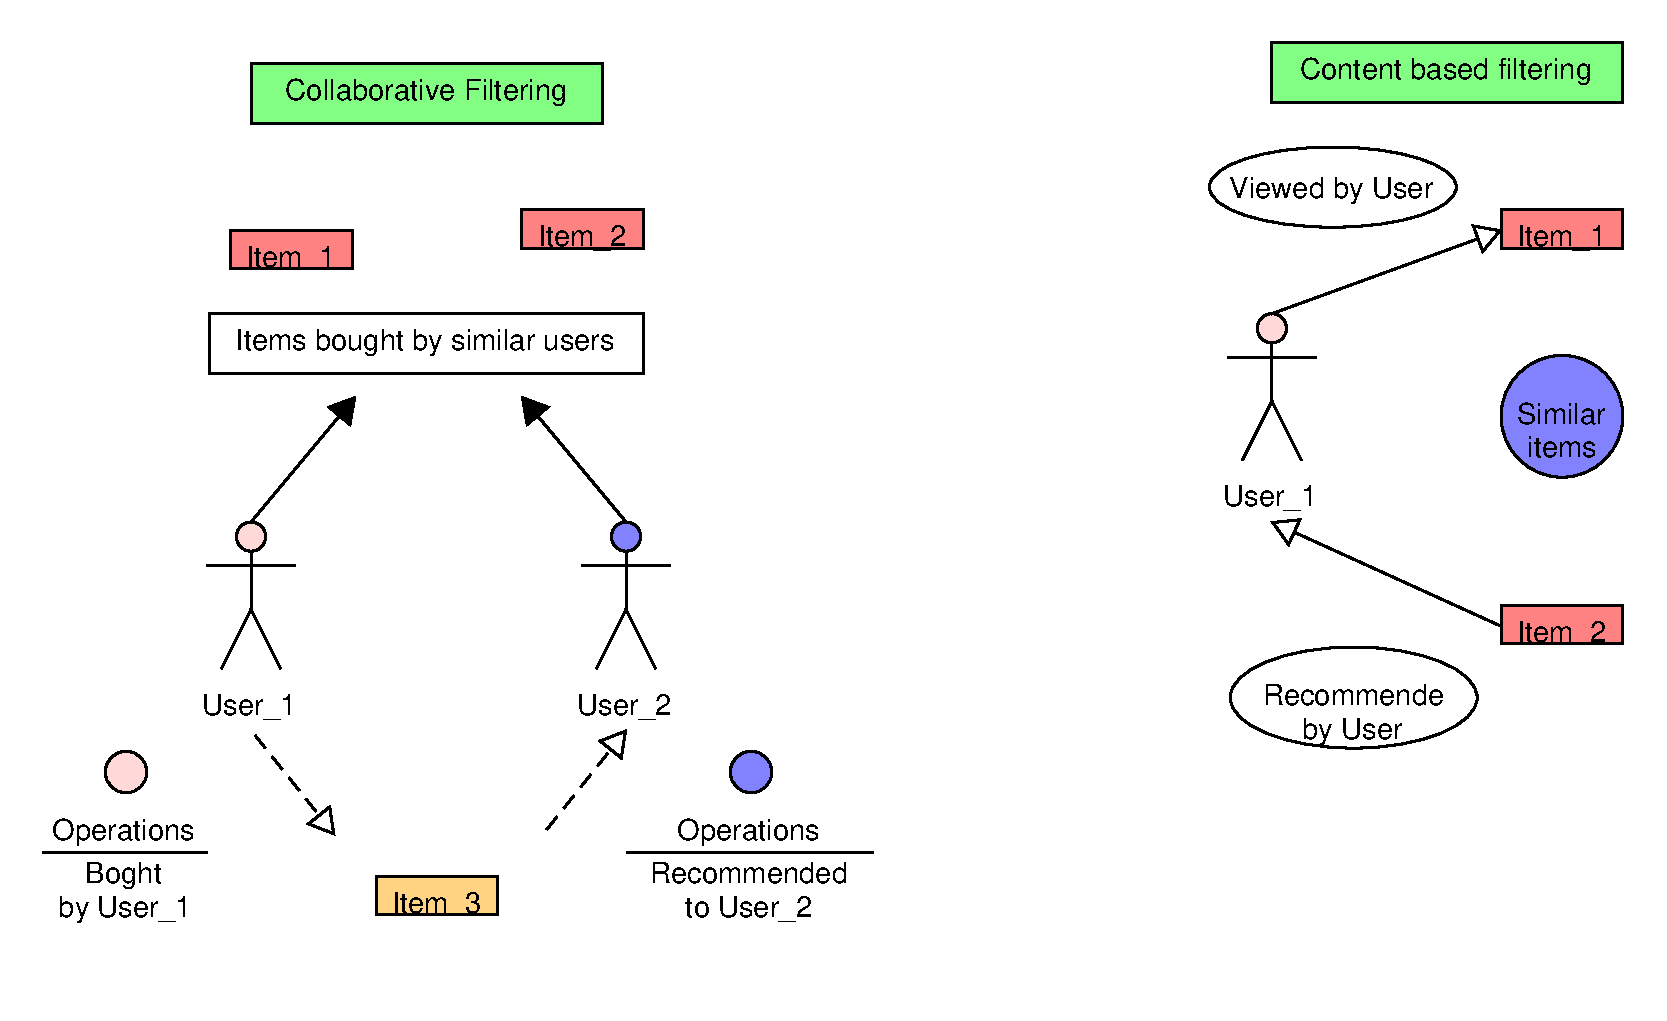
\includegraphics[width=0.6\textwidth]{Images/Filtering_pdf.pdf} % Adjust width as needed
  \caption{Prvý obrázok UX/UI.}
\end{figure}

\begin{figure}[h!]
  \centering
  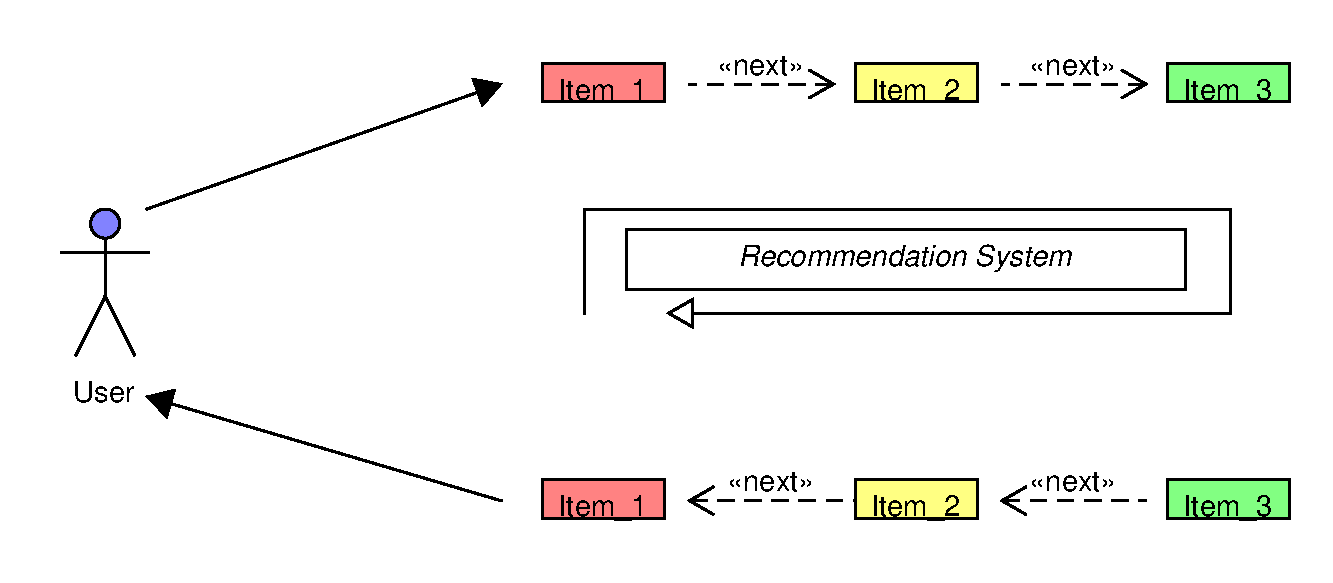
\includegraphics[width=0.6\textwidth]{Images/RecommendationSystem_pdf.pdf} % Adjust width as needed
  \caption{Druhý obrázok UX/UI.}
\end{figure}


\section{Úvod}
Úvod do problematiky algoritmov odporúčania na platforme Netflix.
Krátke zhrnutie vplyvu technológií a umelé inteligencie na naše rozhodovanie pri výbere obsahu na sledovanie.

\section{Technológie a Umelá inteligencia v Netflix}
Vplyv technológií a umelé inteligencie na dnešné odporúčacie systémy.
Vývoj algoritmov odporúčania na Netflixu a ich súčasný stav.

\section{Typy Odporúčaní na Netflix}
Detailné vysvetlenie rôznych typov odporúčaní (napr. Odporúčané pre vás, Trendy, Nové vydania) a ich úloha v navigácii používateľov.

\section{Filtračné algoritmy}
Porovnanie a vysvetlenie algoritmov collaborative filtering a filtrovania na základe obsahu.
Vplyv hodnotení a správania používateľov na úspešnosť algoritmov.

\section{Systémy Hodnotenia}
Prehľad o rôznych systémoch hodnotenia (Personalizované hodnotenie videa, Top-N Ranking, Rebríčky obľúbených filmov, Zoznam zaujímavého obsahu na neskoršie sledovanie).
Ako tieto systémy prispievajú k osobnej skúsenosti používateľov.

\section{Typy Údajov v Netflix}
Kategórie základných údajov (interakcie používateľa, histórie sledovania).
Význam dodatočných informácií (žánre, korelačné údaje, informácie o obsahu).

\section{Vplyv špecifickejších informácií}
Analýza vplyvu denného času, používaného zariadenia a priemerného času sledovania na odporúčacie algoritmy Netflixu.

\section{Záver}
Zhodnotenie významu algoritmov odporúčania pre Netflix a ich vplyv na používateľskú skúsenosť.
Diskusia o budúcnosti vývoja algoritmov odporúčania.
\begin{thebibliography}{9}

\bibitem{netflixRecAlgorithm} 
\href{https://stratoflow.com/how-netflix-recommendation-algorithm-work/}{Netflix Recommendation Algorithm}.  

\bibitem{netflixAlgorithm} 
\href{https://recostream.com/blog/recommendation-system-netflix}{Netflix Algorithm}.  

\end{thebibliography}

\end{document}
